\section{$\text{H}_2$/$\text{O}_2$ reaction kinetics: higher-dimensional case}
\label{sec:app}

For the high-dimensional case, we aim to investigate the impact of the uncertain
pre-exponents ($A_i$'s) as well as the activation energies ($E_{a,i}$'s) on ignition 
delay during the H$_2$/O$_2$ reaction.  Prior distributions for $A_i$'s were considered
to be the same as provided earlier in section~\ref{sec:method}. The $E_{a,i}$'s for all
reactions except $\mathcal{R}_6$ -- $\mathcal{R}_9$ and $\mathcal{R}_{13}$ (due to 
zero nominal values for $E_a$)
were considered to be uncertain and uniformly distributed in the interval: 
$[0.99E_{a,i}^\ast, 1.01E_{a,i}^\ast]$. Hence, the total number of uncertain rate parameters
is 33. The nominal values, $E_{a,i}^\ast$
corresponding to the different reaction rates are provided in~\cite{Yetter:1991}. 

\subsection{Computing the active subspace}

The active subspace was computed using the iterative procedure outlined in Algorithm~\ref{alg:grad}.
The convergence of the eigenvectors
was examined by tracking $\max(\delta \hat{\mat{W}}_{1,j}^{(i)})$, plotted in 
Figure~\ref{fig:conv_app} (right). In Figure~\ref{fig:conv_app} (left), individual
components of the converged eigenvector are illustrated. The convergence was established using
a $\tau$ value of 0.02. Finite difference was used to compute model gradients at 40 samples in
the input domain. Hence, a total of 1360 model evaluations were required for this purpose.  
%
\begin{figure}[htbp]
 \begin{center}
  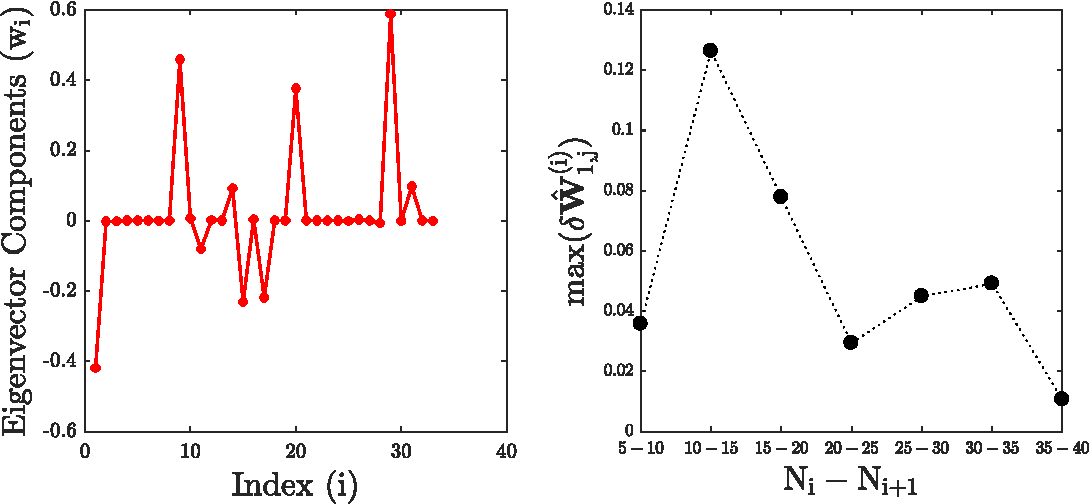
\includegraphics[width=0.8\textwidth]{./Figures/eigv10}
\caption{Left: An illustrative comparison of individual components of the converged dominant eigenvector,
obtained using the perturbation-based strategy. Right: The quantity,  
$\max(\delta \hat{\mat{W}}_{1,j}^{(i)})$
is plotted for successive iterations to illustrate the convergence behavior.}
\label{fig:conv_app}
\end{center}
\end{figure}
%
 
In Figure~\ref{fig:hd} (left), we illustrate the resulting eigenvalue spectrum. The second eigenvalue is
found to be roughly two orders of magnitude smaller than the first, indicating that the active subspace
is 1-dimensional. This is further confirmed by the SSP plots in Figure~\ref{fig:hd} (right), generated
using both, perturbation-based and regression-based strategies. 
%
\begin{figure}[htbp]
 \begin{center}
   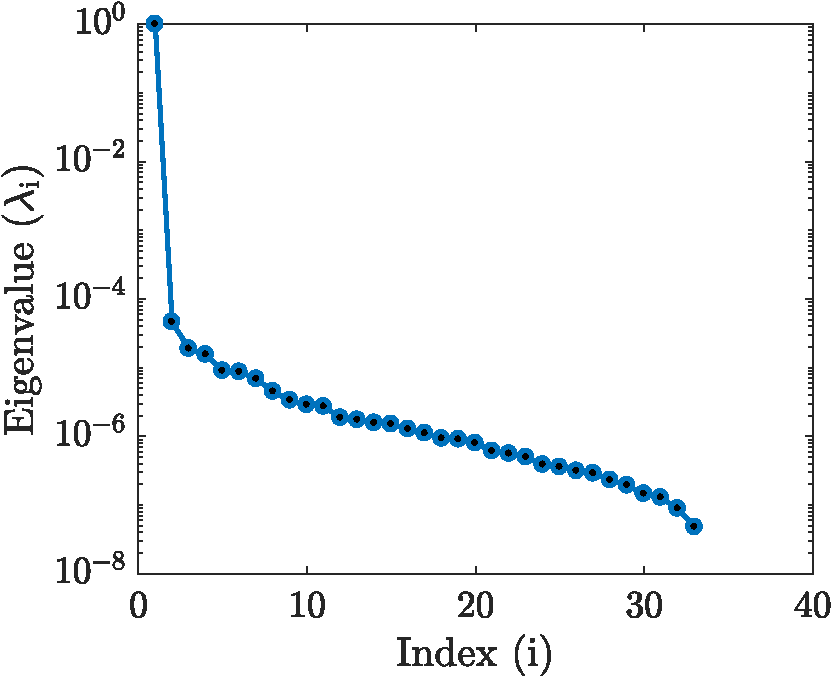
\includegraphics[width=0.45\textwidth]{./Figures/eig_33D}
   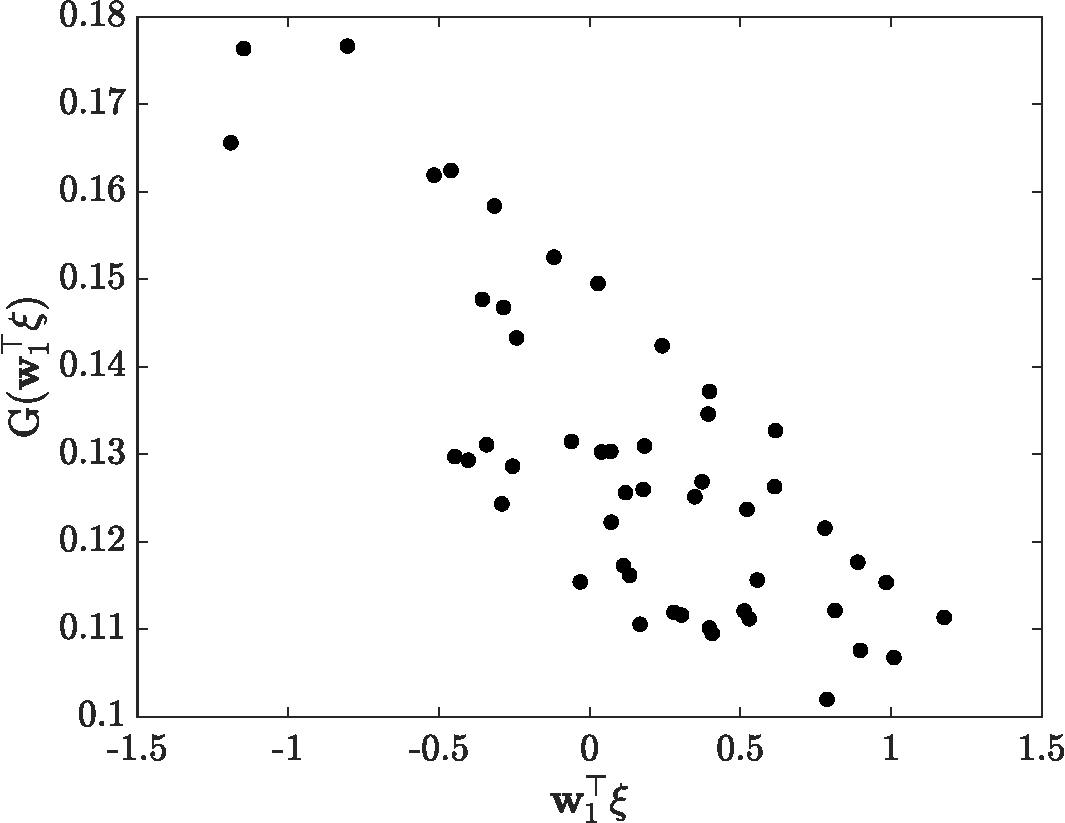
\includegraphics[width=0.45\textwidth]{./Figures/ssp_33D}
\caption{Left: Eigenvalue spectrum of $\hat{\mat{C}}$. Right: SSP of the computed active subspace, and the
corresponding 1-D linear fit.} 
\label{fig:hd}
\end{center}
\end{figure}
%
Specifically
in the case of perturbation-based strategy, the SSP is observed to exhibit a linear variation that
is reasonably
captured by the corresponding straight-line fit, $\tilde{G}$, constructed using the sequence of steps
outlined in Section~\ref{sub:ac}.
On the other hand, the SSP constructed using the regression-based strategy
is relatively more scattered. Consequently, the two surrogates (straight-line fits) are observed to exhibit a
discrepancy unlike our earlier observation for the 19-dimensional problem in Figure~\ref{fig:comp_ssp}. 

\subsection{Surrogate Verification}
\label{sub:verify}

The 1-dimensional surrogate ($\tilde{G}$) shown in Figure~\ref{fig:hd}~(right) is investigated
for its accuracy as well as the ability to capture the uncertainty in the
model output in two ways. Firstly, we estimate the relative L-2 norm of the discrepancy~($\varepsilon_d$)
between estimates of ignition delay in the case of H$_2$/O$_2$ reaction, obtained using the 
model output and the surrogate in the following equation:
%
\be
\varepsilon_d = \frac{\|G(\bm{\xi}) - \tilde{G}(\bm{\xi})\|_2}{\|G(\bm{\xi})\|_2}
\ee
%
Model evaluations ($G$) at 10$^{4}$ samples in the input domain were used to evaluate $\varepsilon_d$. 
It was estimated to be 1.35$\times10^{-2}$ and 1.02$\times10^{-1}$
using $\tilde{G}$ based on the perturbation-based and the regression-based strategies respectively. Hence,
$\varepsilon_d$ was found to increase by an order of magnitude when using the regression-based strategy.
Therefore, in the norm-sense, it can be said that the 1-dimensional surrogate in the active subspace, obtained
using the perturbation-based approach is remarkably accurate with a relative error of less than 1.5$\%$, whereas
the regression-based approach resulted in a relative error of about 10$\%$.

Secondly, we verified the accuracy of the two surrogates in a probabilistic setting. In particular, we compared 
probability density functions (PDFs) obtained using the true set of model evaluations, and 1-dimensional
surrogates ($\tilde{G}$'s) from the two strategies, in Figure~\ref{fig:pdf_33D}. Note that the three PDFs were evaluated 
using the same set of 10$^4$ samples in the cross-validation set. 
%
\begin{figure}[htbp]
\begin{center}
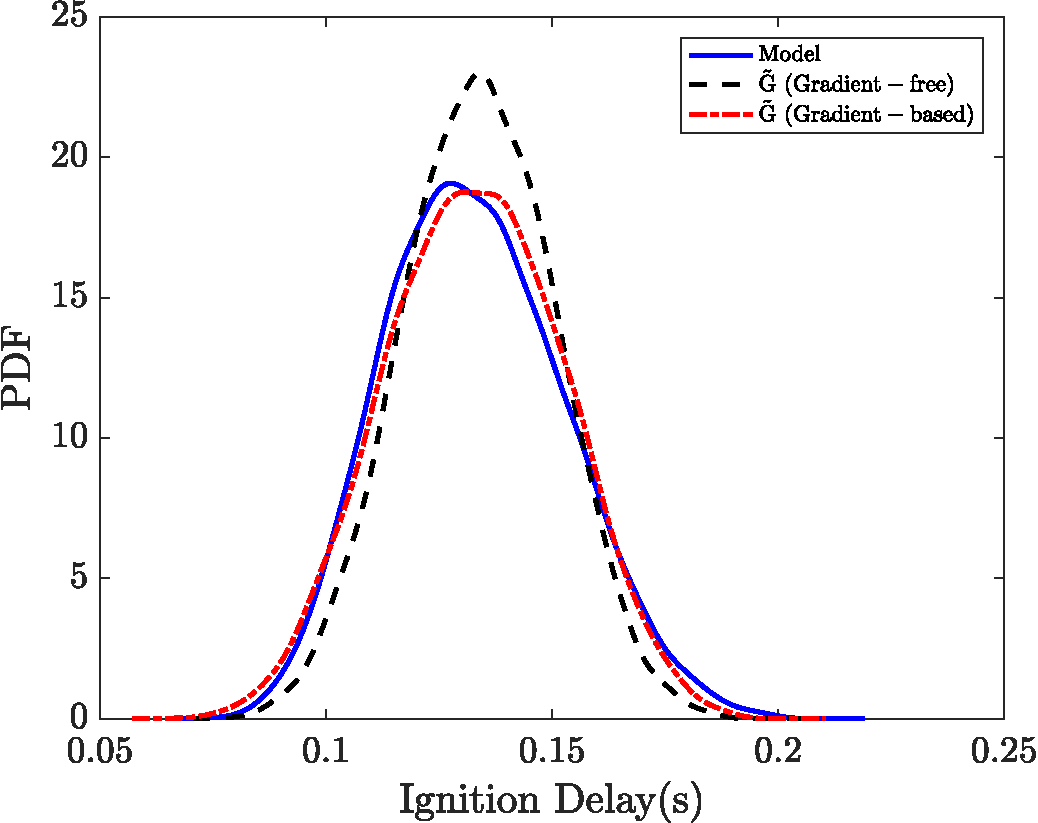
\includegraphics[width=3.0in]{./Figures/pdf_comp_id_1e4}
\end{center} 
\caption{A comparison of the PDFs of ignition delay, obtained using model 
evaluations (solid line) and 1-dimensional surrogates using the regression-based strategy (dashed line) and the
perturbation-based strategy (dashed-dotted line). The same set of 10$^4$ samples in the cross-validation set were 
used in each case.}
\label{fig:pdf_33D}
\end{figure}
%
%
%\begin{figure}[htbp]
% \begin{center}
%  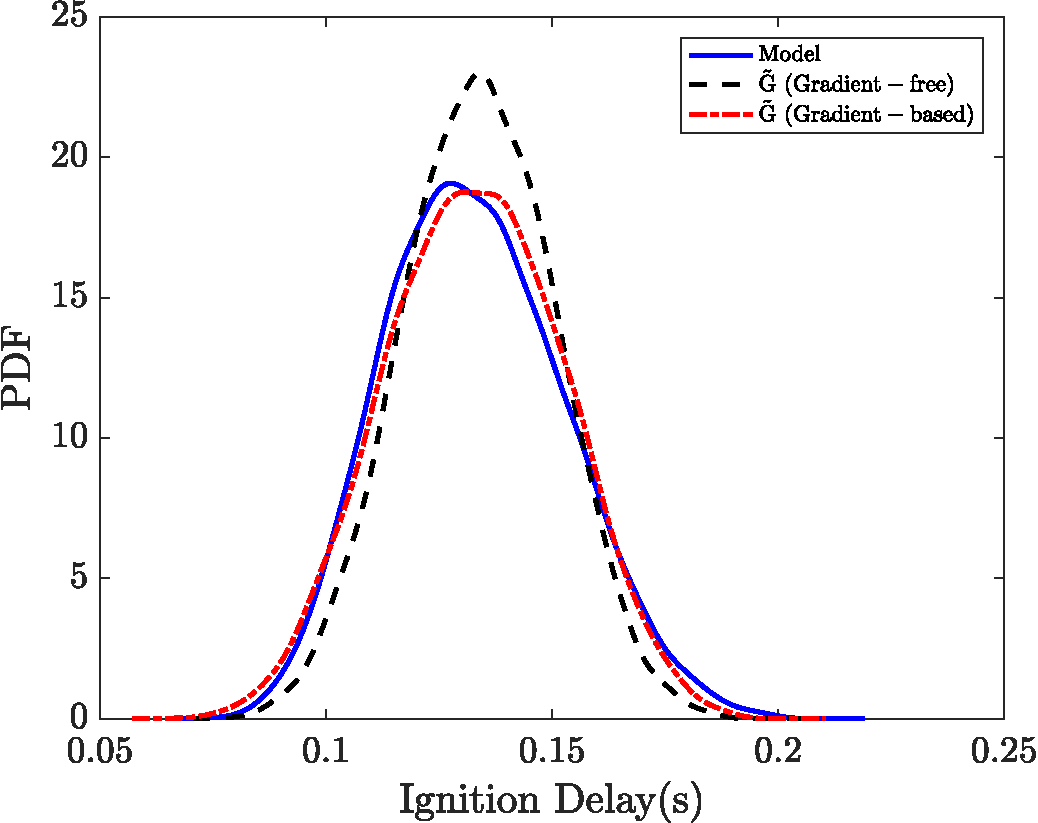
\includegraphics[width=0.45\textwidth]{./Figures/pdf_comp_id_1e4}
%\caption{A comparison of the PDFs of ignition delay, obtained using model evaluations (solid line) and
%1-dimensional surrogates using the gradient-free approach (dashed line) and the gradient-based approach
%(dashed-dotted line). The same set of 10$^4$ samples in the cross-validation set were used in each case.}
%\label{fig:pdf_33D}
%\end{center}
%\end{figure}
%
The PDFs based on the model evaluations and the perturbation-based strategy are nearly identical, confirming
the existence of a 1-dimensional active subspace as well as the accuracy of this strategy. 
On the other hand, although the PDF obtained using the regression-based strategy is observed to show
consistency with the true PDF in the modal
estimate, it clearly underestimates the spread in the ignition delay. Specific values of the mean and the standard 
deviation in each case are provided in Table~\ref{tab:stats}. 
%
\begin{table}[htbp]
\begin{center}
\begin{tabular}{ccc}
\toprule
$\textbf{Distribution}$ & $\mu$ & $\sigma$ \\ 
\bottomrule
$G$~(Model) & 0.133 & 0.0198 \\
$\tilde{G}$~(Perturbation-based) & 0.133 & 0.0196 \\
$\tilde{G}$~(Regression-based) & 0.133 & 0.0167 \\
\bottomrule
\end{tabular}
\caption{The mean ($\mu$), and the standard deviation ($\sigma$), computed using the model ($G$), and
the surrogate ($\tilde{G}$) based on the two strategies at 10$^4$ samples in the cross-validation
set.}
\label{tab:stats}
\end{center}
\end{table}
%
The three PDFs are found to be
consistent in their prediction of mean value of the ignition delay.  The standard deviation estimates based on model
evaluations and the perturbation-based strategy are found to be in close agreement, whereas, it  is accurately
 estimated in the case of regression-based strategy only upto the first significant digit. 

\subsection{GSA consistency check}

The normalized activity scores ($\tilde{\nu}_{i,r}$) based on the dominant eigenspace using the two
approaches (gradient-based and gradient-free) are compared with the total Sobol' indices
in Figure~\ref{fig:as_33D}. Note that the Sobol' indices were computed using the verified
1-dimensional surrogate in the active subspace for the gradient-based approach. 
%
\begin{figure}[htbp]
 \begin{center}
  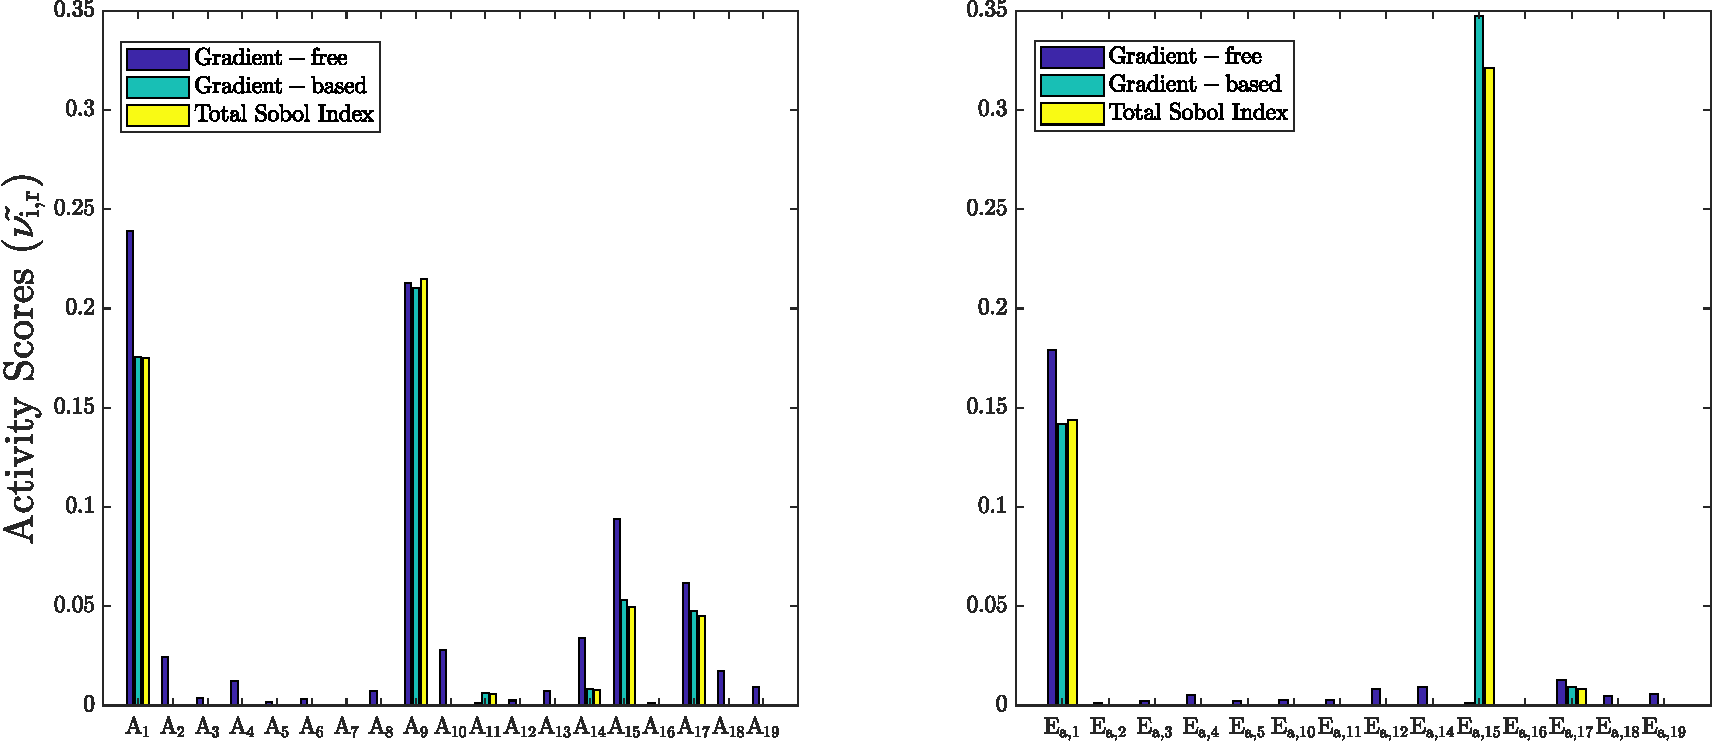
\includegraphics[width=0.8\textwidth]{./Figures/as_33D_new}
\caption{A bar-graph illustrating individual activity scores for the uncertain $A_i$' (left) and $E_{a,i}$'s (right).}
\label{fig:as_33D}
\end{center}
\end{figure}
%
Several useful inferences can be drawn from the above plot. Firstly, the total Sobol indices are found to be
consistent
with the normalized activity scores evaluated using the gradient-based approach. The gradient-free
approach yields consistent results for the $A_i$'s, but it does not capture the sensitivity associated with
$E_{a,15}$. This is because numerical errors are incurred when approximating
the model gradients using the regression-based approximation in the gradient-free case. 
Secondly, our findings indicate that   
the ignition delay is predominantly sensitive towards $A_1$, $A_9$, $E_{a,1}$, and $E_{a,15}$ and 
moderately sensitive towards $A_{15}$ and $A_{17}$. Sensitivity towards the remaining uncertain inputs is
found to be low or negligible. 
%Note that this observation can also be exploited for reducing the 
%dimensionality of the problem from 33 inputs to 4-6 inputs depending upon the required level of accuracy.
%The sensitivity-driven dimension reduction for uncertainty quantification has been
%discussed in our earlier effort~\cite{Vohra:2018}. In this work, however, we focus on dimension reduction using the active 
%subspace approach which is shown to yield even greater scope for dimension reduction i.e. from 33 to 1. Furthermore, we have
%shown that the dominant eigenspace can be used to approximate global sensitivity measures with no additional effort.

